\documentclass[11pt,a4paper,twoside]{report} %impostazione della classe del codumento correttamente
\usepackage[english]{babel}%sillabazione
\usepackage[utf8]{inputenc}%accenti

%per stampare
%\usepackage[inner=4cm,	outer=1cm,		bottom=1.8cm,		top=1.8cm]	{geometry}

%per leggere su monitor
\usepackage[inner=2cm,	outer=2cm,		bottom=1.8cm,		top=1.8cm]	{geometry}


\usepackage[titles]{tocloft} %table of content

\usepackage{hyperref}%link alle varie sezioni e ai capitoli
\hypersetup{
    colorlinks,
    citecolor=black,
    filecolor=black,
    linkcolor=black,
    urlcolor=black
}

\usepackage[parfill]{parskip} %le nuov5e righe non iniziano indentate

\usepackage{caption}

\newcommand*\E{\`E\ } %comando \E per fare la e accentata maiuscola

%pacchetti non configurati direttamente
\usepackage{graphicx,wrapfig,epigraph,titlesec,lipsum,xcolor,anyfontsize}
\usepackage{bold-extra}



\graphicspath{{img/},{../}}
\usepackage{listings}
\usepackage{courier}
\usepackage{multicol}
\lstset{
	frame=single,
	basicstyle=\ttfamily
}


%stile di titoli di chapter section e subsection

\newcommand{\hsp}{\hspace{6pt}}

\titleformat{\chapter}[block]
	{\fontsize{35pt}{0pt}\sffamily\bfseries}
	{\fontsize{60pt}{0pt}\sffamily\thechapter\hsp\textcolor{gray75}{$|$}\hsp}
	{0pt}{\fontsize{30pt}{0pt}\bfseries}

\titlespacing{\chapter}{0pt}{-30pt}{30pt}


\usepackage{tikz}
\usepackage{epigraph,anyfontsize}


\renewcommand\epigraphflush{flushright}
\renewcommand\epigraphsize{\normalsize}
\setlength\epigraphwidth{0.7\textwidth}

\definecolor{titlepagecolor}{cmyk}{.10,.60,1,.20}

\definecolor{gray75}{gray}{0.75}

\makeatletter
\def\printauthor{%
	{\Large \sffamily\bfseries \@author}}
\def\printtitle{%
	{	\sffamily\bfseries \noindent

		\fontsize{30pt}{60pt} \selectfont \@title}
}
\def\printdate{%
	{ \sffamily \large \@date}}

\makeatother


% The following code is borrowed from: http://tex.stackexchange.com/a/86310/10898

\newcommand\titlepagedecoration{%
	\begin{tikzpicture}[remember picture,overlay,shorten >= -10pt]

	\coordinate (aux1) at ([yshift=-15pt]current page.north east);
	\coordinate (aux2) at ([yshift=-410pt]current page.north east);
	\coordinate (aux3) at ([xshift=-4.5cm]current page.north east);
	\coordinate (aux4) at ([yshift=-150pt]current page.north east);

	\begin{scope}[titlepagecolor!40,line width=12pt,rounded corners=12pt]
	\draw
	(aux1) -- coordinate (a)
	++(225:5) --
	++(-45:5.1) coordinate (b);
	\draw[shorten <= -10pt]
	(aux3) --
	(a) --
	(aux1);
	\draw[opacity=0.6,titlepagecolor,shorten <= -10pt]
	(b) --
	++(225:2.2) --
	++(-45:2.2);
	\end{scope}
	\draw[titlepagecolor,line width=8pt,rounded corners=8pt,shorten <= -10pt]
	(aux4) --
	++(225:0.8) --
	++(-45:0.8);
	\begin{scope}[titlepagecolor!70,line width=6pt,rounded corners=8pt]
	\draw[shorten <= -10pt]
	(aux2) --
	++(225:3) coordinate[pos=0.45] (c) --
	++(-45:3.1);
	\draw
	(aux2) --
	(c) --
	++(135:2.5) --
	++(45:2.5) --
	++(-45:2.5) coordinate[pos=0.3] (d);
	\draw
	(d) -- +(45:1);
	\end{scope}
	\end{tikzpicture}%
}

\renewcommand\maketitle{
	\begin{titlepage}

		\noindent
		\printtitle\par
		%\epigraph{ NOME }
		%{\textsc{Sviluppo di una Web Application in JSP}}
		\null\vfill
		\vspace*{1cm}
		\noindent
		\hfill
		\begin{minipage}{0.55\linewidth}
			\begin{flushright}
				\printauthor

				\vspace{10pt}

				\printdate
			\end{flushright}
		\end{minipage}
		%
		\begin{minipage}{0.02\linewidth}
			\rule{1pt}{65pt}
		\end{minipage}
		\titlepagedecoration
	\end{titlepage}

}














\author{Matteo Battilana - 180209\\Massimo Girondi - 178114\\Daniele Isoni - 181839}

\title{Progetto di \\Introduzione alla \\programmazione per il Web}
\date{Versione del \today}
\begin{document}
\maketitle
\clearpage\null\newpage
\tableofcontents
\clearpage\null\newpage

\chapter{Tecnologie utilizzate}

Il progetto è stato realizzato con Java in versione 7, coadiuvato dalle librerie per lo sviluppo Web tra cui JSP e JSTL.

L'interfaccia Web è stata sviluppata attraverso Twitter Bootstrap 3, con JQuery e HTML5.

Il database scelto è stato MySQL, data la grande affidabilità. Rappresenta il giusto compromesso tra flessibilità e velocità.

All'interno dell'applicazione sono integrate altre librerie JavaScript, tutte liberamente scaricabili, e alcune chiamate alle API di Google Maps, in particolare per l'autocompletamento dei campi e per la visualizzazione della mappa.

Il sito è responsive e supporta la localizzazione mediante le tecnologie offerte da Java Web (resourceBundle e Format Library).

La maggior parte delle pagine sono realizzate mediante una coppia servlet-JSP, soluzione che permette di separare il codice dalla struttura visiva e ottimizza l'uso delle risorse. Sono inoltre presenti alcuni filtri per poter controllare l'accesso a determinate pagine.


Lo sviluppo dell'applicazione è stato gestito facendo uso di Git e GitHub, i quali ci hanno concesso di sviluppare autonomamente diverse parti del progetto, er poi unirle insieme, oltre a mantenere la ``storia'' delle modifiche e fornire un repository centralizzato per il codice.
Abbiamo utilizzato un workflow a branch: ogni componente del gruppo sviluppava su un branch diverso e, al termine delle modifiche, questo veniva unito al master mediante \texttt{merge}.




\chapter{Installazione}
Per poter installare l'applicazione è necessario seguire i seguenti passi:
\begin{enumerate}

\item Ripristinare il database e i dati presenti nella cartella \texttt{DB/DBUtils/}.
\item Copiare la cartella \texttt{DB/DBUtils/UploadedContent da copiare} nella cartella \\\texttt{\textbf{catalina.base}/UploadedContent}.
La posizione della cartella \texttt{\textbf{catalina.base}} varia da installazione a installazione e, solitamente, si trova nel percorso \texttt{/opt/tomcat/bin/} (Linux e Mac) o analoghi.
\item Definire quindi le proprie impostazioni nel file \\\texttt{PROJECT/BuyHub/src/main/resources/config.properties}.
\item Modificare le impostazioni per il proprio server di posta elettronica nel file\\ \texttt{PROJECT/BuyHub/src/main/java/it/unitn/buyhub/utils/Mailer.java}. In particolare, togliere il commento dalla riga 67 per abilitare l'invio e immetere le proprie credenziali nelle righe 109-126. Per avere i dettagli su come configurare il client email, contattare il provider del servizio.
\item \E quindi possibile eserguire l'applicazione all'interno di Apache TomCat o GlassFish.
\end{enumerate}

\chapter{Database}

Il database scelto è stato MariaDB, una variante di MySQL. Abbiamo scelto questa distribuzione grazie alla semplice installazione realizzata mediante XAMPP, con il quale viene installato anche PHPMyAdmin, una comoda interfaccia di gestione del database. Un altro punto a favore di questo DBMS è la totale compatibilità con MySQL (tutte le query funzionano anche su un normale database MySQL) e la velocità, oltre alla stabilità e la diffusione pressochè globale.

\section{Entities DAO - Data Access Object}
Per ogni entità presente che necessita di interazioni con il Database è stato creato il relativo DAO per permetterne una corretta interazione. Il DAO (Data Access Object) è un pattern architetturale che ha come scopo quello di separare le logiche di business da quelle di accesso ai dati. L’idea alla base di questo pattern è quello di descrivere le operazioni necessarie per la persistenza del modello in un’interfaccia e di implementare la logica specifica di accesso ai dati in apposite classi. (Fonte: html.it)

\begin{center}
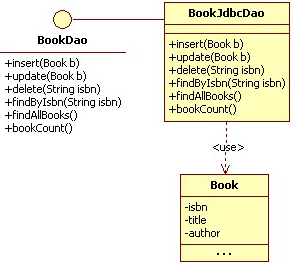
\includegraphics[width=0.3\linewidth]{img/dao}
\end{center}

\section{Struttura del database}

Il database è stato strutturato per essere il più semplice possibile nell'utilizzo. \E stato strutturato secondo le principali regole di design relazionale, utilizzando chiavi esterne e indici. Sono state inoltre incluse alcune tabelle e alcuni campi superflui, utili per un'implementazione futura. Di seguito una rapida descrizione delle tabelle:
\begin{itemize}
  \item \textbf{users}: questa è la tabella principale del database, attorno alla quale è costruito tutto il resto. Descrive ogni singolo utente e ne determina anche i privilegi (con un campo intero: 0 se l'utente è disabilitato, 1 se è un utente normale, 2 se è un utente abilitato alla gestione di un negozio, 3 se è un amministratore). Per scelta implementativa un amministratore non può avere un negozio e un negozio può avere solo un utente ad esso collegato.
  \item \textbf{shops}: questa tabella contiene i dati dei singoli negozi. Il campo \texttt{validity} descrive l'abilitazione o meno del negozio, mentre i campi \texttt{shipment} e \texttt{shipment\_costs} determinano se la spedizione è disponibile (se il primo campo è vuoto significa che non lo è) e il costo della stessa.
  \item \textbf{coordinates}: in questa tabella sono inseriti i singoli punti vendita. Ogni negozio può infatti avere più punti vendita sul territorio, ognuno con un proprio indirizzo e un poprio orario di apertura
  \item \textbf{products}: questa tabella contiene tutti i dati dei prodotti in vendita. La categoria è determinata con un ID numerico, che viene poi convertito in testo attraverso il codice Java. Una descrizione delle categorie si trova nei file della lingua e come appendice a questo documento.
  \item \textbf{pictures}: questa tabella contiene i dati delle foto caricate attraverso il sito. Nell'implementazione attuale solo i campi \texttt{id}, \texttt{name} e \texttt{path} sono utilizzati, gli altri sono pensati per una futura implementazione.
  \item \textbf{pictures\_products} e \textbf{pictures\_shops} : mediante questa relazione possiamo collegare le foto ai prodotti e ai negozi.
  \item \textbf{reviews}: questa tabella contiene i dati delle recensioni dei prodotti. Per scelta  implementativa è presente un indice sulla coppia \texttt{(id\_product, id\_creator)} che impedisce ad un utente la creazione di più di una recensione sullo stesso oggetto.
  \item \textbf{pictures\_reviews}: questa tabella non è al momento utilizzata. Servirebbe per implementare la possibilità di allegare foto  alle recensioni.
  \item \textbf{orders}: in questa tabella vengono salvati i dati di tutti gli ordini. Viene salvato anche il metodo e il costo di spedizione, dato che nel tempo potrebbero variare (ma un ordine fatto nel passato non deve essere influenzato da questi cambiamenti).
  \item \textbf{orders\_products}: mediante questa tabella possiamo salvare i prodotti associati ad un ordine. Oltre alla quantità viene salvato anche il prezzo perchè, come per i costi di spedizione, potrebbero variare nel tempo.
  \item \textbf{tickets}: un ticket è una segnalazione ad un negozio relativa ad un ordine. In questa tabella vengono salvati i ticket aperti in modo tale da sapere se a un dato ordine è associato un ticket.
  \item \textbf{messages}: all'interno di questa relazione sono salvati tutti i messagi associati a un ticket.
  \item \textbf{notifications}: questa entità contiene i dati delle notifiche che vengono inviate agli utenti. Queste sono generate da degli eventi (segnalazione ticket, apertura negozio, ...) e sono mostrate agli utenti nella barra principale.
\end{itemize}

\begin{center}
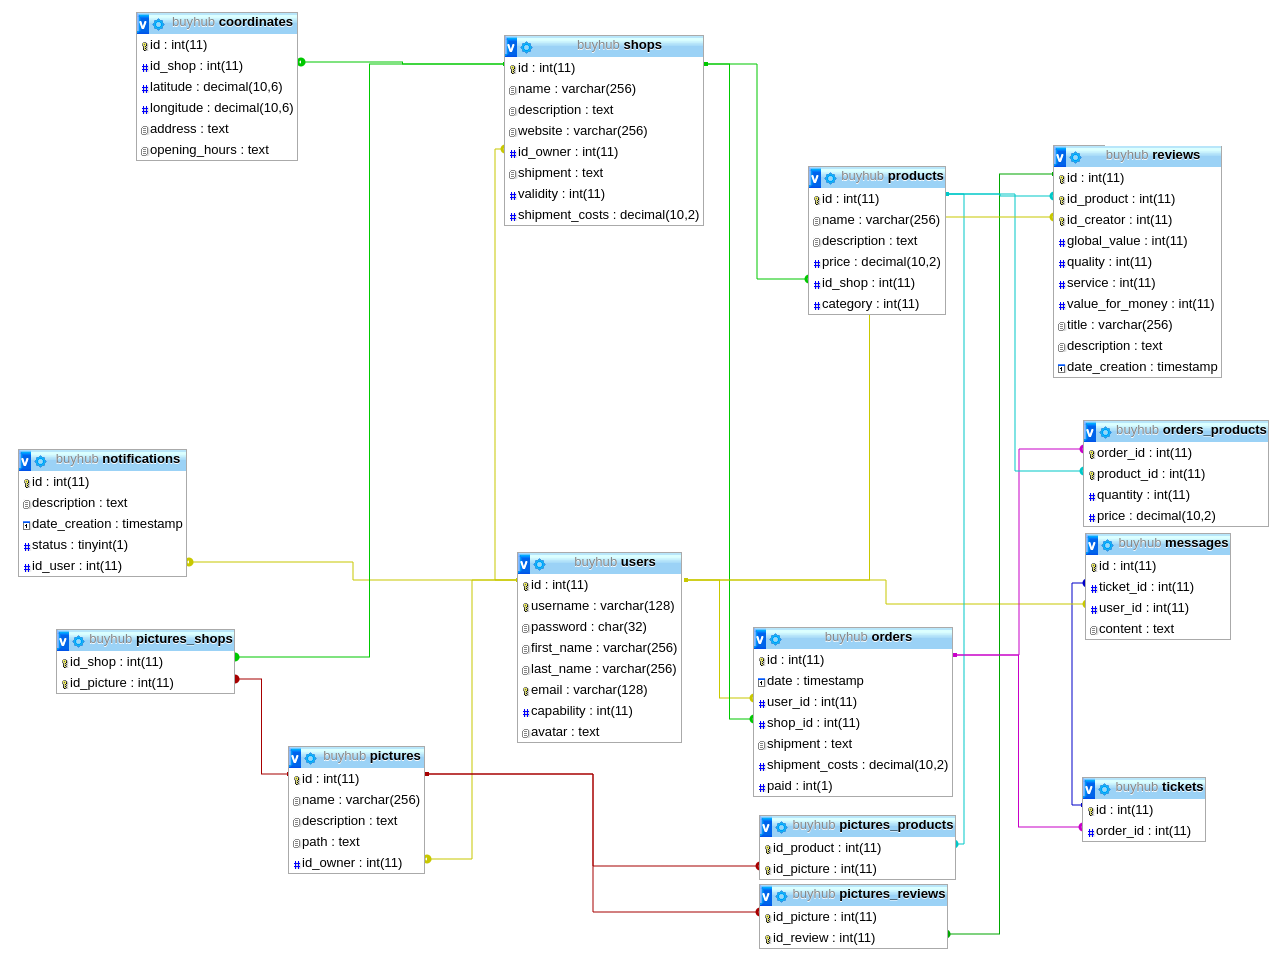
\includegraphics[width= \linewidth]{er}
\end{center}


\section{Popolazione di test}
Il DataBase di test (\texttt{DB/DBUtils/data.sql}) è così formato:
\begin{itemize}

  \item 62 punti vendita associati a 31 negozi (almeno un punto vendita a negozio)
  \item 336 prodotti totali inseriti, distribuiti equamente in tutti i negozi (almeno un prodotto per negozio)
  \item 327 fotografie (di cui 302 associate a prodotti)
  \item 122 utenti, ognuno con il proprio avatar
  \item 2298 recensioni, almeno una per prodotto e 7 in media per prodotto

\end{itemize}

Tutti i campi utilizzati nella nostra applicazione sono stati riempiti con valori verosimili, prelevati dal Web mediante degli script Python, alcuni dei quali presenti nella cartella \texttt{DB/DBUtils/scripts}, pertanto non rispettano assolutamente il nostro pensiero e non ci assumiamo nessuna responsabilità del contenuto degli stessi.

I punti vendita sono stati distribuiti casualmente attorno a 6 città (Vicenza, Trento, Bologna, Milano, Udine, Verona). La loro distribuzione è riassunta nell'immagine seguente:
\begin{center}
  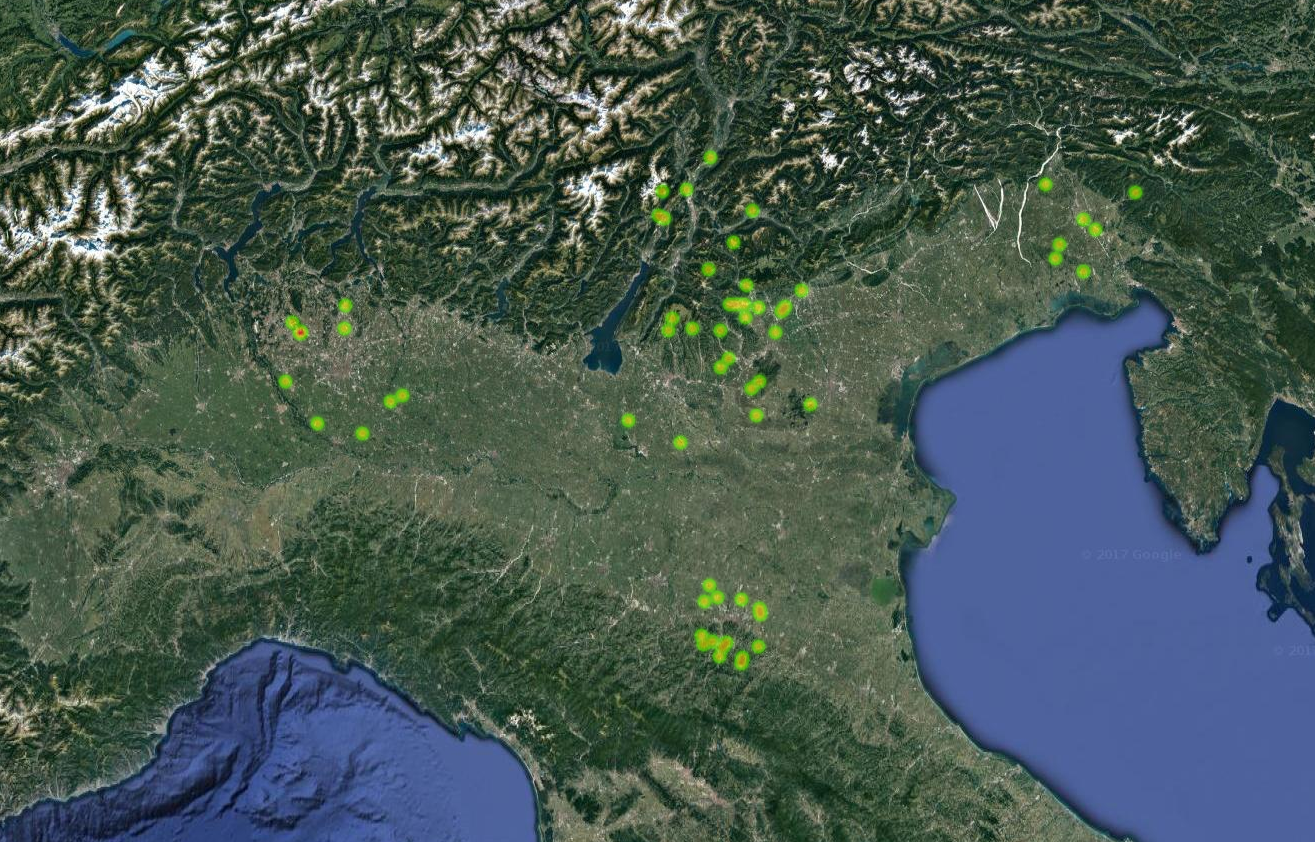
\includegraphics[width=10cm]{heatmap}
\end{center}


\chapter{Autocompletamento}

\section{Barra di ricerca}
L'autocompletamento presente nella barra di ricerca è stato realizzato mediante la libreria JavaScript  \textbf{bootstrap-ajax-typeahead}, la quale recupera i suggerimenti per l'autocompletamento dalla servlet AutoCompleteServlet mediante richieste Ajax, a cui la servlet rispone in formato JSON.

La servlet effettua una ricerca per similarità (secondo l'algoritmo di Jaro-Winkler) all'interno di una lista, la quale viene caricata all'avvio dell'applicazione analizzando i nomi dei prodotti presenti nel database e aggiornata a intervalli prestabiliti (ogni 30 minuti) mediante le classi Executors e ScheduledExecutorService presenti all'interno di Java stesso.

Abbiamo scelto questa implementazione per evitare di sovraccaricare il database eseguendo una query a ogni richiesta di autocompletamento (e quindi a ogni tasto premuto).
Un'altra opzione, poi scartata, era aggiornare la lista dell'autocompletamento a ogni modifica della tabella dei prodotti, ma questo avrebbe rallentato ogni operazione sulla tabella stessa.

L'algoritmo di Jaro-Winkler è utilizzato anche durante la scansione del database, per evitare di inserire nella lista dei suggerimenti titoli doppi o troppo simili (ad esempio ``frigo'' e ``frigorifero'') dato che questi verrebbero comunque selezionati al momento della ricerca, dove è applicata ancora una volta la similarità.

\section{Indirizzo}
L'autocompletamento presente nel form di creazione di un nuovo negozio per l'indirizzo è stato utilizzato mediante la libreria JavaScript \textbf{Google Maps API}. Queste API permettono tramite chiamate asincrone di ricevere i suggerimenti i quali vengono mostrati mediante un dropdown. Una volta fatta la scelta vengono riempiti i campi del bean con indirizzo completo, e coordinate (latitudine e longitudine).

\chapter{Risultati della ricerca}
La ricerca tra i prodotti è realizzata mediante una servlet che elabora la richiesta e restituisce la lista dei prodotti sottoforma di JSON. L'unico parametro obbligatorio è \texttt{q} che rappresenta la query di ricerca.
I parametri opzionali sono:
\begin{itemize}
  \item \texttt{p}: la pagina desiderata (nel caso di  una ricerca multipagina)
  \item \texttt{s}: il metodo di ordinamento dei risultati, di default alfabetico (0), alfagetico inverso(1), prezzo crescente (2), prezzo decrescente(3), valutazione decrescente(4),  numero recensioni decrescente(5).
  \item \texttt{c}: la categoria
  \item \texttt{min} e \texttt{max}: gli estremi dei prezzi.
  \item \texttt{minRev}: il minimo del valore delle recensioni.
\end{itemize}
Il controllo sul nome del prodotto e sul range di prezzo è effettuato all'interno del DAO del prodotto (mediante SQL per il prezzo e algoritmo di Jaro-Winkler per il nome), mentre il controllo sulla categoria e sul valore minimo della media delle recensioni è effettuato mediante un predicato invocato dal metodo \texttt{removeIf} della lista prodotti.
Oltre alla lista prodotti nel risultato sono restituiti anche il numero di pagine, il tipo di ordinamento usato e la pagina corrente.


\chapter{Logging}
Il logging, fondamentale per un'applicazione di questo tipo, è stato implementato mediante la libreria Apache Log4j, che consente di gestire in modo molto semplice i vari livelli di log e il salvataggio automatico sul disco.

Abbiamo poi creato un wrapper attorno alla libreria per limitare il più possibile il numero di istruzioni richieste per scrivere un messaggio nel log.

I log vengono salvati nella cartella \texttt{\$CATALINA\_HOME/logs} in file testuali che iniziano con il nome \texttt{BuyHub}.
La cartella \texttt{\$CATALINA\_HOME} è in genere la cartella di installazione di TomCat o GlassFish, ma potrebbe variare in base alla configurazione del sistema.

\chapter{Dettagli implementativi}

\section{Orari di apertura e negozi solo online}
Per semplificare la struttura del DB abbiamo deciso di implementare i vari punti vendita dei negozi come una relazione uno a molti tra \texttt{shop} e \texttt{coordinate}. All'interno della tabella \texttt{coordinate} abbiamo inserito il campo \texttt{opening\_hours} che contiene gli orari del punto vendita, nel caso in cui per il cliente sia disponibile il ritiro in negozio. Nel caso di negozi che effettuano soltanto vendita online questo campo resta vuoto e viene sostituito all'interno della pagina web con un messaggio che specifica le modalità di vendita solo online del negozio.

\section{Carrello}
Il carrello utente, visto come contenitore temporaneo di prodotti da acquistare è stato implementato a livello di \textit{sessione}; questo significa che i prodotti aggiunti in una sessione non saranno salvati sul database e quindi in un futuro login il carrello sarà vuoto.

\chapter{Upload/Download}

L'upload dei file è stato gestito mediante la libreria \texttt{com.oreilly.servlet}, mentre il salvataggio dei file è gestito da alcuni metodi all'interno della classe \texttt{Utility}.

In particolare, il metodo \texttt{saveJPEG} si occupa di salvare un immagine, dandogli un nome casuale basato su un UUID, convertendola a JPEG, mediante la libreria ImageIO, integrata in Java.
Purtroppo questa libreria non gestisce correttamente le trasparenze nelle immagini PNG, e al momento, non è ancora stata trovata una soluzione per ovviare a questo problema, in quanto non è possibile dedurre se questo errore di codifica è avvenuto o no.

I file vengono poi salvati in una cartella definita all'interno del file \texttt{config.properties}, nel quale è possibile inserire sia un path relativo (in base alla propria cartella \texttt{catalina.base}), oppure un percorso assoluto, che verrà automaticamente interpretato e utilizzato per il salvataggio.

Il dowload avviene mediante la servlet \texttt{UploadedContentServlet}, che risponde alle richieste che arrivano alle url del tipo \texttt{/UploadedContent/*}, in modo tale da simulare a tutti gli effeti una cartella. Il file richiesto viene inviato in modalità ``inline'', e con il relativo MIME impostato. Nel caso il file non sia presente nel disco, viene restituita un'immagine che indica la non presenza del file.

La scelta di utilizzare questo sistema è stata piuttosto ardua, in quanto, non volendo usare path assoluti, l'unica opzione per caricare un file direttamente con Java, era caricarlo nella cartella di esecuzione (la \texttt{contextPath}). Nel momento in cui però sarebbe avvenuto un redeploy tutti i file sarebbero stati cancellati, oltre al fatto che alcuni server Java non permettono la scrittura nella \texttt{contextPath}. Altri server, invece, mantengono direttamente tutto il \texttt{.war} dell'applicazione in RAM, senza creare una cartella nel disco rigido, e creare cartelle locali alla \texttt{contextPath} in questo contesto è abbastanza sconsigliato (aumenterebbe a dismisura l'uso di RAM).

Un'altra soluzione, volendo realizzare un prodotto per il mondo reale, sono i CDN, in particolare quelli specifici per le immagini, come cloudinary.com o imgix.com. Questi servizi, però, sono in genere a pagamento e non permettono il controllo completo delle proprie immagini. Per questi motivi la scelta è ricaduta nel caricare le immagini in un path locale alla cartella di esecuzione, ma esterno al \texttt{contextPath}, in modo da preservare i file tra le diverse esecuzioni e deploy dell'applicazione.




\chapter{Verifica dell'account}

Quando un utente si registra al sito, è prevista una conferma della registrazione attraverso la mail, onde evitare account fasulli. All'interno della mail viene inserito un link che contiene un codice speciale che abilita l'utente all'accesso.

In particolare, tale codice è composto dall'ID utente e dall'Hash della password, grazie ai quali è possibile identificare l'utente e, data la bassa probabilità di indovinare l'MD5, rende difficile un eventuale attacco.

Questo codice è poi cifrato mediante AES128 secondo una chiave segreta presente nel server, che ci consente quindi di essere \textit{praticamente} certi che un utente smaliziato riesca ad accedere a un account non proprio. Per poter inviare correttamente il risultato mediante una URL il codice è codificato prima in Base64 e poi attraverso la funzione \texttt{URLEncode} di Java. Il codice è quindi così formato:
\[
    URLEncode( Base64( AES( \mbox{id}\$MD5(\mbox{password}))))
\]

\chapter{Homepage}
Nella homepage vengono visualizzati gli ultimi 10 prodotti inseriti nel database, sulla base dell'ID. Sopra agli ultimi prodotti è presente uno slider con alcune immagini, contenute nella cartella \texttt{images/slider\_images}. Lo slider supporta la localizzazione: carica, mediante un taghandler, tutti i file presenti nella cartella corrispondente alla lingua selezionata. Ad esempio, se la lingua è italiano, caricherà tutte le immagini presenti nella cartella \texttt{images/slider\_images/it/}.


\chapter{Mail}
Il sito consente l'invio automatico di email. Queste vengono inviate facendo uso della classe \\\texttt{it.unitn.buyhub.utils.Mailer}.
All'interno di questa classe sono implemntati diversi componenti:
\begin{itemize}
  \item La sottoclasse \texttt{RunnableMailer}, che implementa l'interfaccia \texttt{Runnable}. Questa classe permette di inviare una mail in maniera asincrona e multithread. Questo significa che durante l'invio della mail l'applicazione non deve attendere ma può eseguire altre operazione (ad esempio renderizzare la pagina di avvenuto pagamento).
  \item Il metodo \texttt{mail} che invoca \texttt{RunnableMailer}, inviando l'email, e aggiunge al log le informazioni della mail.
  \item Il metodo \texttt{mailToAdmins} che invoca il già noto metodo \texttt{mail} per ogni amministratore presente nel database.
  \item Il metodo \texttt{sendMail} che esegue l'invio vero e proprio. Questo metodo è anche chiamato all'interno di \texttt{RunnableMailer}.
  \item \texttt{BuildMail}, un metodo che ``costruisce'' la mail in formato HTML. Viene chiamato all'interno di \texttt{sendMail}.
\end{itemize}

L'invio della mail è effettuato mediante la classe \texttt{javax.mail}, che effettua un collegamento \texttt{SMTP} e consegna il messaggio al server. Le credenziali di accesso al server sono ``hardcoded'' all'interno della classe, perciò è richiesto modificarle prima di eseguire l'applicazione.

Abbiamo scelto di salvare le credenziali in questo modo in quanto ogni provider di posta utilizza parametri diversi per l'invio e realizzare un codice funzionante per ogni provider avrebbe causato problemi di sicurezza (ad esempio la connessione cifrata non è supportata da tutti i provider, sarebbe stato quindi necessario disabilitarla).




\chapter{Altri capitoli}
\chapter{Conclusioni}

\chapter{Appendice}
\section{Categorie prodotti}


\begin{itemize}

\item \textbf{0:} Abbigliamento e accessori
\item \textbf{1:} Alimentari e cura della casa
\item \textbf{2:} Arte e antiquariato
\item \textbf{3:} Auto, moto e altri veicoli
\item \textbf{4:} Bellezza e salute
\item \textbf{5:} Biglietti ed eventi
\item \textbf{6:} Cancelleria e prodotti per ufficio
\item \textbf{7:} Casa, arredamento e bricolage
\item \textbf{8:} Collezionismo
\item \textbf{9:} Commercio e Industria
\item \textbf{10:} Elettrodomestici
\item \textbf{11:} Elettronica
\item \textbf{12:} Film e DVD
\item \textbf{13:} Fotografia e video
\item \textbf{14:} Francobolli
\item \textbf{15:} Fumetti
\item \textbf{16:} Giardino e arredamento esterni
\item \textbf{17:} Giocattoli e modellismo
\item \textbf{18:} Gioielli
\item \textbf{19:} Handmade
\item \textbf{20:} Illuminazione
\item \textbf{21:} Infanzia e premaman
\item \textbf{22:} Informatica
\item \textbf{23:} Libri e riviste
\item \textbf{24:} Monete e banconote
\item \textbf{25:} Musica, CD e vinili
\item \textbf{26:} Nautica e imbarcazioni
\item \textbf{27:} Orologi
\item \textbf{28:} Orologi e gioielli
\item \textbf{29:} Prima infanzia
\item \textbf{30:} Prodotti per animali domestici
\item \textbf{31:} Salute e cura della persona
\item \textbf{32:} Sport e tempo libero
\item \textbf{33:} Sport e viaggi
\item \textbf{34:} Strumenti musicali e DJ
\item \textbf{35:} Telefonia fissa e mobile
\item \textbf{36:} TV, audio e video
\item \textbf{37:} Valigeria
\item \textbf{38:} Veicoli: ricambi e accessori
\item \textbf{39:} Videogiochi
\item \textbf{40:} Videogiochi e console
\item \textbf{41:} Vini, caffè e gastronomia
\end{itemize}


\end{document}
